\section{Feladat leírása}

A projekt célja egy Parkinson-kóros betegek rehabilitációját támogató mobilalkalmazás fejlesztése volt.
A betegségre jellemző motoros tünetek (például a testtartási instabilitás vagy a járászavarok) miatt a
fizikai rehabilitáció kiemelt fontosságú.
Az alkalmazás célja ennek megfelelően nem orvosi diagnózis felállítása, hanem a rehabilitációs
folyamat informatikai támogatása és a gyakorlatok során keletkező adatok strukturált kezelése.

A megoldás a Sensoria által kifejlesztett viselhető szenzor (okoszokni) adatait dolgozza fel.
A szenzor a gyakorlatok közben valós időben szolgáltat információt a sarok, a lábfej és a
lábujjak terheléséről, valamint a láb x, y és z irányú gyorsulásáról, a zokni összeállítása
az \ref{fig:sock}. ábrán látható.

\begin{wrapfigure}{r}{0.4\textwidth}
    \centering
    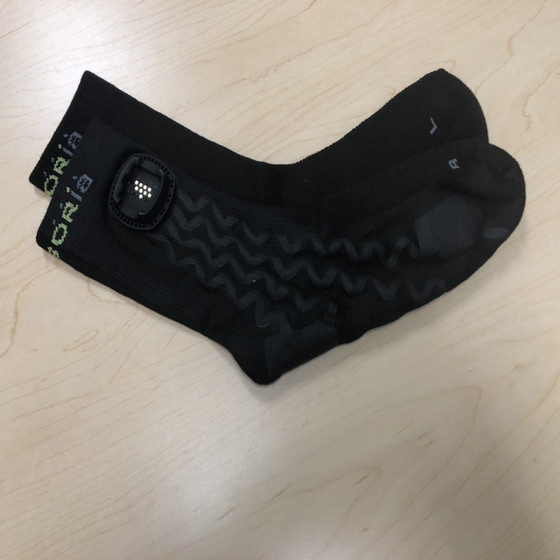
\includegraphics[width=0.4\textwidth]{images/sock}
    \caption{A Sensoria okoszokni \cite{sensoria2016walk}, látható a bluetooth csatlakozó
    helye a zokni szárán és a talp részén a szenzorok elhelyezkedése.}
    \label{fig:sock}
\end{wrapfigure}

Ezeket az adatokat az alkalmazás fogadja, feldolgozza, majd az adott munkamenethez kapcsolva
tárolja. A mérési folyamatot videós útmutató is kiegészíti, amely lehetőséget ad a
gyakorlatok megtekintésére és megfelelő végrehajtására.


A tervezett rendszernek több fő funkciót kellett megvalósítania.
Ezek közé tartozott az előre rögzített gyakorlatok listázása és kiválasztása,
a mérési munkamenet indítása és lezárása, a Sensoria okoszokniból érkező szenzoradatok kezelése,
a videós komponensek integrálása, valamint az eredmények áttekinthető megjelenítése.
Fontos szempont volt az is, hogy a korábban rögzített munkamenetek később visszakereshetők
és megtekinthetők legyenek.


A fejlesztés során az egyik tervezési szempont volt a moduláris felépítés.
Ennek köszönhetően az alkalmazás később új rehabilitációs feladatokkal,
további mérési módszerekkel vagy új elemzési funkciókkal is bővíthető maradhat.


















